




\section{Motivation}
%%%%%%%%%%%%%%%%%%%%%%%%%%%%%%%%%%%%%%%%%%%%%%%%%%%%%%%%%%%%%%%%%%%%%%
\begin{frame}[label=intro30]{Two routes to KT}
 \begin{center}%\includegraphics[height=1.2cm]{COPL}%
  %\hspace{2cm}
  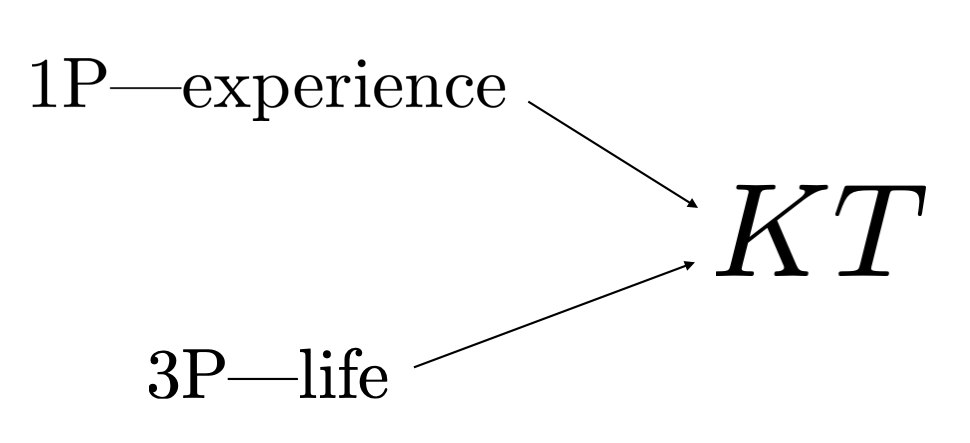
\includegraphics[height=5.2cm]{img/KT.png}
  \end{center}
\end{frame}
%%%%%%%%%%%%%%%%%%%%%%%%%%%%%%%%%%%%%%%%%%%%%%%%%%%%%%%%%%%%%%%%%%%%%%
\begin{frame}[label=intro]{The subjective route to KT: Experience (1P)}
	We start from the fact of {\em experience}---the first person (1P), subjective standpoint \citep{Ruffini2017}.  \vfill
	
	Meditation, psychedelics, religious experience (e.g., Buddhism) suggest that experience can be pure/primordial, free from mental constructs such as the ego.\vfill
	
	From the self-evidence of our own experience, the ``what it's like to be'', we assume that  primordial experience does not  allow for or require prior causes.\vfill
	
    \begin{alertblock}{Warning:  We assume {\em there exists experience.} } 
	KT does not address the hard problem of consciousness.  
	\end{alertblock}
	

\end{frame}

%%%%%%%%%%%%%%%%%%%%%%%%%%%%%%%%%%%%%%%%%%%%%%%%%%%%%%%%%%%%%%%%%%%%%%
\begin{frame}[label=intro2]{Structured experience (\SEP)}
 We aim to build a theory around the notion of 
{\em structured experience}---where {\em mathematics} and experience meet.  \vfill

{\bf Mathematics:}  The science of structure, order, and relation  \cite{gray_2010}.  \vfill

%Following the phenomenological tradition, w
We observe that  experience is {\em structured}: at least during wakefulness, there is a spatial, temporal, and conceptual organization of our 1P experience of the world (inc. {\em self}). \vfill

	\begin{definition}[{\em structured experience} (\SEP)]
The phenomenal structure of consciousness  encompassing both sensory qualia and the spatial, temporal, and conceptual organization of our experience  \citep{VanGulick:2016aa}. 
	\end{definition}

	

\end{frame}

%%%%%%%%%%%%%%%%%%%%%%%%%%%%%%%%%%%%%%%%%%%%%%%%%%%%%%%%%%%%%%%%%%%%%%
\begin{frame}[label=intro3]{Scientific strategy for the study of \SEP}
This definition of \SEP can be empirically explored in reporting humans, and  we   aim to characterize it with methods  applicable to a broad range of systems.  \vfill

  The strategy will be to quantify the structure of experience from {\bf 1P reports}  in humans and attempt to associate it with 3P data (e.g., EEG, fMRI, or behavior) using mechanistic insights derived from neuroscience and mathematics --- \textbf{Computational neurophenomenology}.  \vfill
  
  We can then study (3P) other systems (non-reporting humans, other living species or artificial agents) %. \vfill
  %
  %With  bases for comparison  of the state and behavior of an artificial agent and that of an \SEP-reporting human, we
  for an educated guess about the agent's \SEP.

\end{frame}

%%%%%%%%%%%%%%%%%%%%%%%%%%%%%%%%%%%%%%%%%%%%%%%%%%%%%%%%%%%%%%%%%%%%%%
\begin{frame}[label=intro4]{The objective route to KT (3P): persistence and life}
We can also start by attempting to define what {\em life} is.\vfill

What remains after the passage of eons must rightfully be called a {\em persistent pattern}.\vfill

There may be several types of such patterns. Some seem rather  impervious to the world, such as protons.  \vfill

\begin{definition}[Life]
Patterns that readily interact but persist by partly capturing  structure in the world they inhabit  to stay or replicate (homeo- and meta-homeostasis).  \end{definition}\vfill

 {\bf The connection with the first viewpoint is that, in KT, this {generalized definition of \em life is what is capable of \SEP}}. \vfill 
 
 As part of our program, we should study the algorithmics of the emergence of life. 
\end{frame}

%%%%%%%%%%%%%%%%%%%%%%%%%%%%%%%%%%%%%


%\section{AIT and Kolmogorov complexity}

%\subsection{List styles}

% \subsubsection{Itemize}

% \begin{frame}[label=S]\frametitle{ddd} 
% 	\begin{itemize}
% 		\item Item 1
% 		\item Item 2
% 		\begin{itemize}
% 			\item Sub item 1
% 			\item Sub item 2
% 			\begin{itemize}
% 				\item Sub sub sub item 1
% 				\item Sub sub sub item 2
% 			\end{itemize}
% 			\item Sub item 3
% 		\end{itemize}
% 		\item Item 3
% 	\end{itemize}
% \end{frame}

% \subsubsection{Enumerate}

% \begin{frame}[label=enumerate]\frametitle{Enumerate sample} 
% 	\begin{enumerate}
% 		\item Item 1
% 		\item Item 2
% 		\begin{enumerate}
% 			\item Sub item 1
% 			\item Sub item 2
% 			\begin{enumerate}
% 				\item Sub sub sub item 1
% 				\item Sub sub sub item 2
% 			\end{enumerate}
% 			\item Sub item 3
% 		\end{enumerate}
% 		\item Item 3
% 	\end{enumerate}
% \end{frame}

% \subsubsection{Description}

% \begin{frame}[label=description]\frametitle{Description sample}
    
% \begin{description}
% 	\item[Term 1:] Definition 1
% 	\item[Term 2:] Definition 2
% 	\item[Term 3:] Definition 3
% \end{description}

% \end{frame}

% \subsection{Boxes styles}

% \begin{frame}[label=boxes]\frametitle{Boxes Styles}
    
% \begin{block}{Block Title}
% 	Block content
% \end{block}

% \begin{alertblock}{Alert Block Title}
% 	Alert block content
% \end{alertblock}

% \begin{exampleblock}{Example Block Title}
% 	Example block content
% \end{exampleblock}

% \end{frame}

% \subsection{Block environments}

% \begin{frame}[label=environments]\frametitle{Environments Samples}
    
% 	\begin{definition}
% 	Definition content
% 	\end{definition}
  
% 	\begin{example}
% 	Example content
% 	\end{example}

% 	\begin{proof}
% 	Proof content
% 	\end{proof}  
    
% 	\begin{theorem}
% 	Theorem content
% 	\end{theorem}

% \end{frame}


% \subsection{Math}

% \begin{frame}[label=math]\frametitle{Math}
    
% \begin{equation}
% 	V_0 = k_0 \rho \sqrt{n_1^2 - n_2^2}
% \end{equation}

% \end{frame}


% \subsection{Text environments}

% \begin{frame}[label=text]\frametitle{Text Environments}
    
% \begin{quotation}
%   Quotation environment line 1\\
%   Quotation environment line 2
% \end{quotation}
% \begin{quote}
%   Quote environment line 1\\
%   Quote environment line 2
% \end{quote}
% \begin{semiverbatim}
%   Semiverbatim environment
% \end{semiverbatim}
% \begin{verse}
%   Verse environment line 1\\
%   Verse environment line 2
% \end{verse}  

% \end{frame}

% \section{Conclusion}

% \begin{frame}[label=conclu]{Conclusion slide}
% 	That's all folks!
% \end{frame}